%------------------------------%
%% ✎ Dylan (V1) %%%%%%%%% ✅ %%
%% ✎ Alain (V2) %%%%%%%%% ✅ %%
%% ✎ Dylan (V3) %%%%%%%%% ✅ %%
%------------------------------%

\afterpage{%
\afterpage{%

    % Arrière-plan partie II
    \AddToShipoutPictureBG*{%
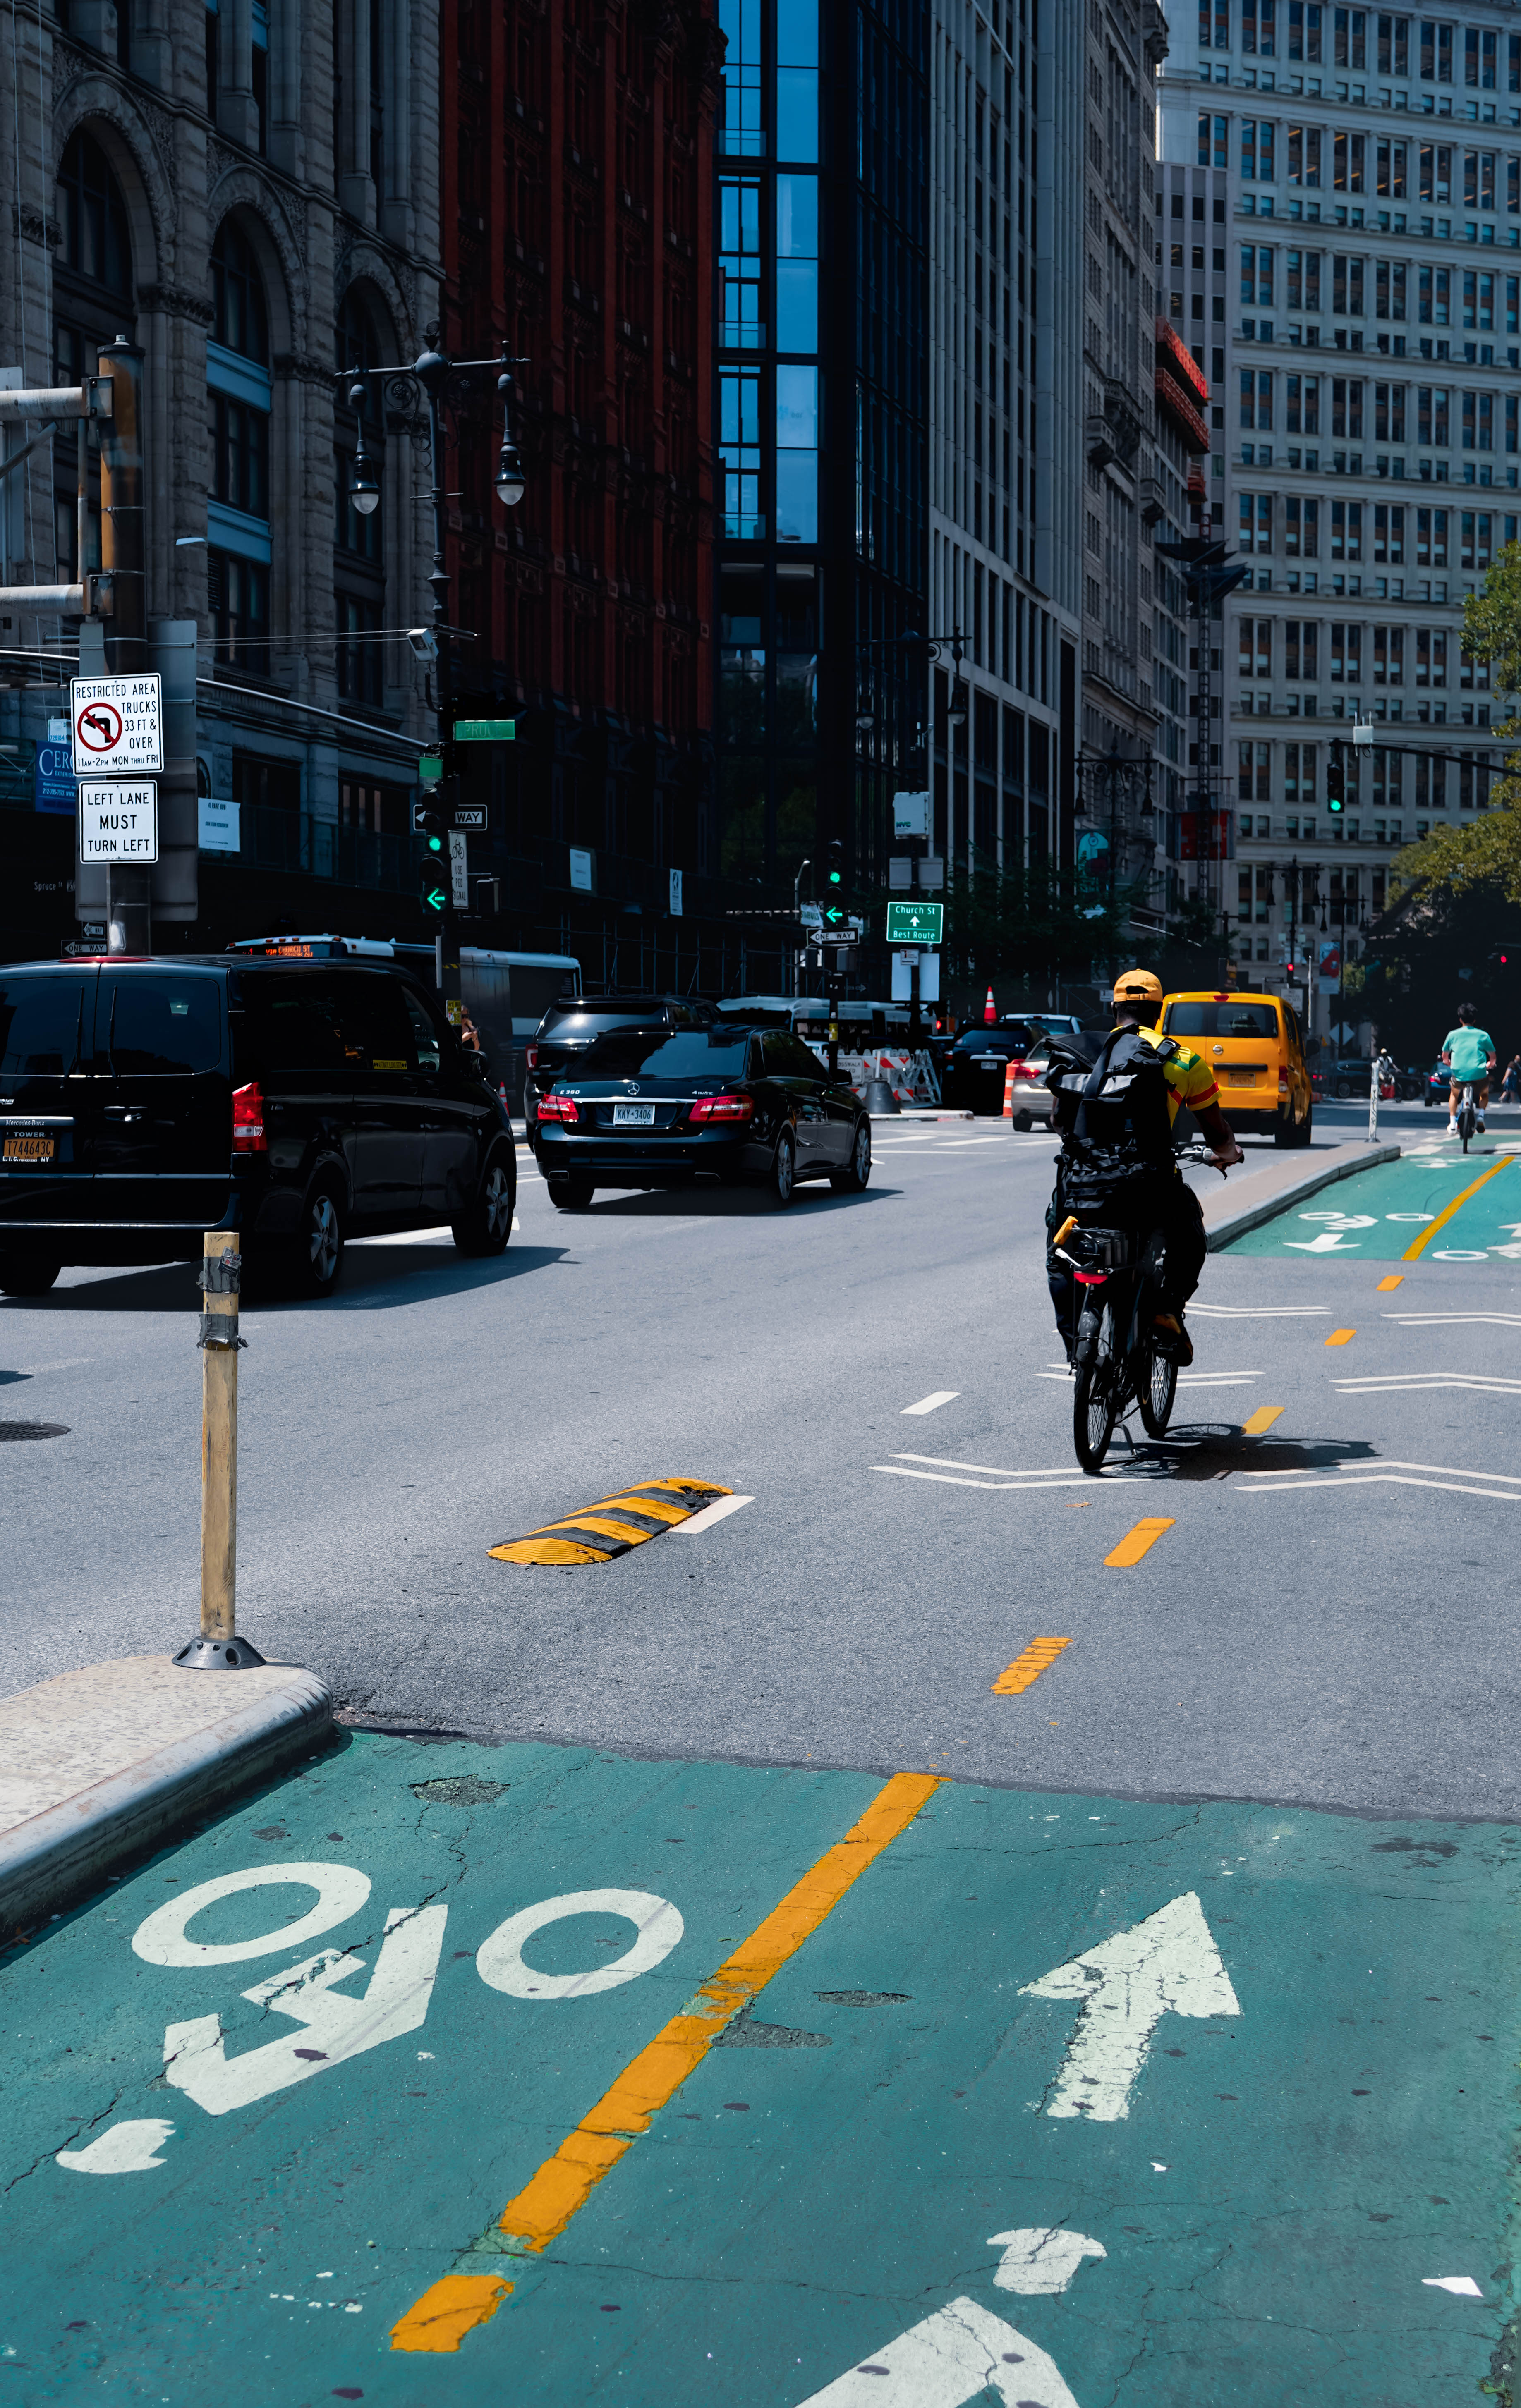
\includegraphics[width=\paperwidth,height=\paperheight]{src/Figures/Arriere_plan/Arriere_plan_Part_2.jpg}
    }

% Rectangle
\AddToShipoutPictureBG*{
  \begin{tikzpicture}[remember picture,overlay]
    \node[fill=white, opacity=0.75, text width=\paperwidth, minimum height=10cm, anchor=north] 
    at ([yshift=-7.7cm]current page.north) {};
  \end{tikzpicture}
}

% Source
\AddToShipoutPictureFG*{
  \AtPageLowerRight{
    \raisebox{1cm}{
      \hspace{16cm}
      
\begin{tikzpicture}
        \node[fill=white, rounded corners=5pt, inner sep=5pt, align=center] {
          \tiny{Photography: \textcolor{blue}{Dylan Moinse (2023)}}
        };
      \end{tikzpicture}
    }
  }
}
}}

\needspace{1\baselineskip} % Reserve space
\part{The Potential for Extending and Transforming Station Districts through the Intermodal Use of Light Individual Mobility
    \label{part2:titre}
    }
    \markboth{Part~II: Intermodal Practices and Accessibility Gains}{}
    \markright{Part~II: Intermodal Practices and Accessibility Gains}{}

% Introduction of Part II
\cleardoublepage
\section*{Introduction of Part~II
    \label{part2:introduction}
    }
    \addcontentsline{toc}{chapter}{Introduction of Part~II}

    % Introduction
\lettrine[lines=3, findent=8pt, nindent=0pt]{\lettrinefont T}{his} second part aims to document and analyze the use of light individual mobility in complementarity with public transport, and to assess its impact on the spatial organization of station districts. It focuses on studying usage dynamics by identifying the factors influencing modal choices, as well as the spatial and territorial effects of light individual mobility on rail spaces and their functional perimeter. By questioning the interactions between infrastructure, mobility practices, and urban structuring, this part aims to shed light on the strategic role of light individual mobility in the evolution of station districts, in relation to the concept of accessibility.%%Translated%%

    % Chapter 4
\textsl{Reporting on Mobility Practices and the Profile of Intermodal Cyclists Using Light Individual Mobility} (\hyperref[objectif-4]{Objective~\(O_4\)}, page~\pageref{objectif-4}). \hyperref[chap4:titre]{The fourth chapter} (page~\pageref{chap4:titre}) is dedicated to studying the use and intermodal practice combining public transport and light individual mobility. It addresses the legitimate question of the proportion of users combining these modes of transport by making use of quantitative observation data to objectively assess the role of light individual mobility within the intermodal transport chain. This study is complemented by an analysis of the questionnaire, which helps to better understand the socio-demographic profile of these social groups, as well as the factors influencing their modal choices and, consequently, the main barriers to adopting these forms of mobility. The qualitative approach based on mobile interviews reveals elements often invisible in quantitative data, discussing the experience and perception of users, highlighting the mobility strategies they employ, and allowing for an understanding of modal trade-offs and motivations. By combining these levels of analysis, this chapter presents a detailed and original portrait of users and their mobility practices, due to the precision of the collected information, which allows for putting into perspective the various existing forms of modal combination.%%Translated%%

    % Chapter 5
\textsl{Decoding the Spatial Implications of Light Individual Mobility in Terms of Intermodal Accessibility} (\hyperref[objectif-5]{Objective~\(O_5\)}, page~\pageref{objectif-5}). \hyperref[chap5:titre]{The fifth chapter} (page~\pageref{chap5:titre}) goes beyond individual mobility practices to explore the territorial effects of the rise in the use, both potential and actual, of light individual mobility in station districts. The goal is to assess how this relationship to proximity transforms the organization of rail spaces and expands accessibility to stations. This chapter employs spatial analysis to measure the accessibility gains generated by the integration of light individual mobility. Inter-nodal and intermodal accessibility have been modeled to compare the functional boundaries of station districts based on the reach of each mode of transport. This approach helps redefine acceptable distances and thus determine the potential for expanding the public transport influence area at the local level, as well as improving rail service within the regional perimeter. In addition, we focused on the route choices of intermodal cyclists to identify preferred paths, based on the presence of infrastructure and types of urban development. This geographic perspective enables us to understand the spatial appropriation logic of mobile individuals and examine the compatibility of current developments with the expressed needs.%%Translated%%